\section{Definição do Problema}

%% Elaborar nesta seção a definição formal do problema, incluindo:
%% - Descrição do problema (priorizar ilustrações e exemplos)
%% - Variáveis de decisão
%% - Função objetivo
%% Sempre que possível, comparar com a literatura
%% Fonte: docs/refs/dissertacao_tex/2-textual/problema.tex
%% Arco: cenário/agenda -> hipóteses -> notação -> restrições R1-R6 -> Z1/Z2 -> gamma.

%%% Frame 2.1 — Contextualização (visual: exemplo de agenda)
\begin{frame}{Contextualização do problema}

    % \vspace{-1cm}
    \begin{center}
        Médicos $\rightarrow$ Clínicas $\rightarrow$ Demanda \\
        {\footnotesize \cite{Rousseau_Pesant_Gendreau_2002,Robinson_Chen_2003}.}
    \end{center}

    \begin{figure}
            \centering
            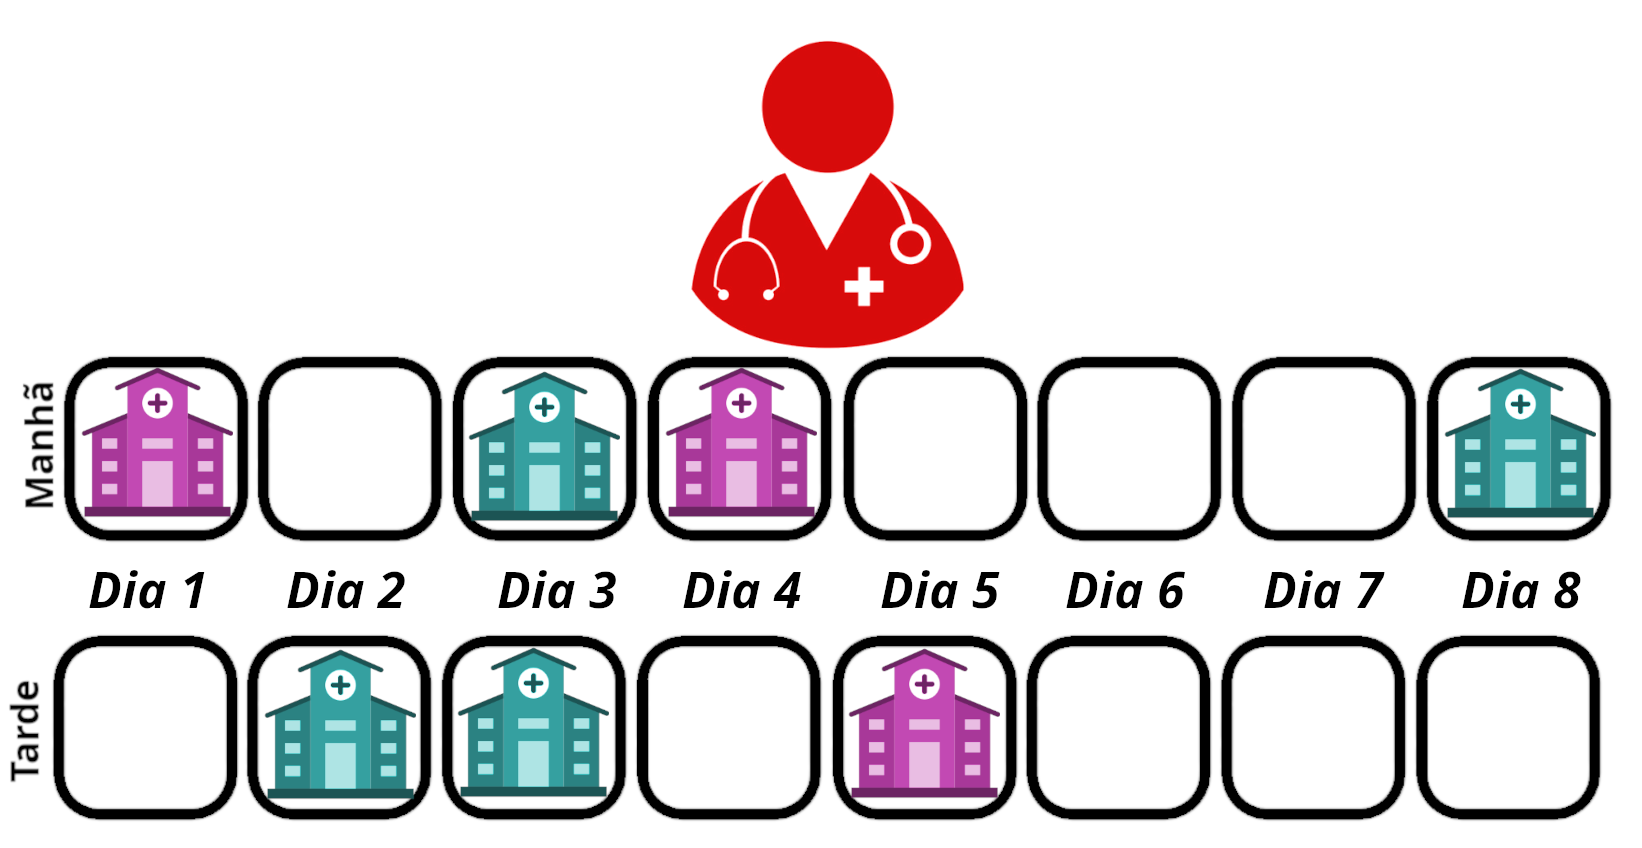
\includegraphics[width=0.6\linewidth]{img/exemplo-schedule-medico.png}
            \caption{Agenda de um médico ao longo do horizonte}
            \label{fig:ex-agenda}
        \end{figure}
    \end{frame}

    \vspace{-1cm}

    % \begin{center}
        
    % \end{center}

%%% Frame 2.2 — Hipóteses de modelagem (tabela)
\begin{frame}{Hipóteses de modelagem}
    \begin{footnotesize}
        \begin{table}
            \centering
            \begin{tabular}{cl}
                \toprule
                \textbf{Hipótese} & \textbf{Descrição} \\
                \midrule
                \textit{H1} & Todas as clínicas atendidas (ao menos cobertura mínima). \\
                \textit{H2} & Médico associado a uma única unidade por dia. \\
                \textit{H3} & Médico associado a uma sala da clínica. \\
                \textit{H4} & Médico realiza exames conforme a demanda da unidade. \\
                \textit{H5} & Atendimentos $-$ demanda $=$ exames não atendidos. \\
                \textit{H6} & Agenda irregular: sem limite de trocas entre clínicas. \\
                \textit{H7} & Condição inicial (histórico) $\rightarrow$ minimizar remanejamentos. \\
                \bottomrule
            \end{tabular}
        \end{table}
    \end{footnotesize}
    % TODO: H1 -> cobertura (R6); H2-H3 -> unicidade (R2-R3); H6-H7 -> trocas (Z2/gamma).
\end{frame}

%%% Frame 2.3 — Notação (conjuntos, parâmetros, variáveis)
\begin{frame}{Notação}
    \begin{small}
        \begin{columns}[T]
            \begin{column}{0.5\textwidth}
                \textbf{Índices e conjuntos}
                \begin{tabular}{ll}
                    $i \in I$ & Médicos \\
                    $u \in U$ & Unidades \\
                    $d \in D$ & Dias \\
                    $t \in T$ & Turnos \\
                    $U_i$     & Unidades de $i$ \\
                    $I_u$     & Médicos de $u$ \\
                \end{tabular}

                \vspace{0.4em}
                \textbf{Parâmetros}
                \begin{tabular}{ll}
                    $e_{udt}$ & Demanda de exames \\
                    $s_{udt}$ & Salas disponíveis \\
                    $q_{idt}$ & Capacidade do médico \\
                    $a_{idt}$ & Disponibilidade $(0/1)$ \\
                    $b_{udt}$ & Há demanda? $(0/1)$ \\
                \end{tabular}
            \end{column}
            \begin{column}{0.5\textwidth}
                \textbf{Variáveis de decisão}
                \begin{tabular}{ll}
                    $x_{iudt}$ & Aloca $i$ em $u$, dia $d$, turno $t$ \\
                    $w_{iud}$  & Aloca $i$ em $u$ no dia $d$ \\
                    $c_{udt}$  & Exames não atendidos \\
                    $z_{id}$   & $i$ trocou de clínica no dia $d$ \\
                \end{tabular}

                \vspace{0.8em}
                \begin{block}{Período}
                    Dia $d$ $\times$ turno $t$ (manhã/tarde); domingo com demanda $0$.
                \end{block}
            \end{column}
        \end{columns}
    \end{small}
\end{frame}

%%% Frame 2.4 — Restrições estruturais R1-R6 (+ chave visual)
\begin{frame}{Restrições estruturais}
    \resizebox{\textwidth}{!}{\begin{minipage}{1.25\textwidth}
        \begin{alignat}{2}
            \sum_{u \in U_i} x_{iudt} &\leq a_{idt} \quad && \forall i \in I, d \in D, t \in T \label{eq:r1} \\
            \sum_{u \in U_i} w_{iud} &\leq 1 \quad && \forall i \in I, d \in D \label{eq:r2} \\
            x_{iudt} &\leq w_{iud} \quad && \forall i \in I, u \in U, d \in D, t \in T \label{eq:r3} \\
            w_{iud} &= 0 \quad && \forall i \in I, u \notin U_i, d \in D \label{eq:r4} \\
            \sum_{i \in I_u} x_{iudt} &\leq s_{udt} \quad && \forall u \in U, d \in D, t \in T \label{eq:r5} \\
            \sum_{i \in I_u} x_{iudt} &\geq b_{udt} \quad && \forall u \in U, d \in D, t \in T \label{eq:r6} \\
            x_{iudt}, w_{iud} &\in \{0,1\} \quad && \forall i, u, d, t \label{eq:dom}
        \end{alignat}
    \end{minipage}}

    \vspace{0.3em}
    {\footnotesize\textbf{Chave:} (\ref{eq:r1})~disponibilidade, (\ref{eq:r2}--\ref{eq:r3})~uma unidade/dia, (\ref{eq:r4}--\ref{eq:r5})~elegibilidade e capacidade de salas, (\ref{eq:r6})~cobertura mínima.}
\end{frame}

%%% Frame 2.5 — Funções objetivo Z1 e Z2 (bi-objetivo)
\begin{frame}{Os "bi"-objetivos do problema}
    \begin{columns}[T]
        \begin{column}{0.54\textwidth}
            $Z_1$ --- \textbf{exames não atendidos} (operacional):
            \begin{alignat}{2}
                c_{udt} &\geq e_{udt} - \!\!\sum_{i \in I_u}\! q_{idt}\, x_{iudt} \label{eq:fo1-r1} \\
                \min\; & \sum_{u,d,t} c_{udt} \label{eq:fo1}
            \end{alignat}

            \vspace{0.5em}
            $Z_2$ --- \textbf{trocas de clínica} (ergonômico):
            \begin{equation}
                \min\; \sum_{i \in I}\sum_{d \in D} z_{id} \label{eq:fo2}
            \end{equation}
        \end{column}
        \begin{column}{0.46\textwidth}
            \begin{figure}
                \centering
                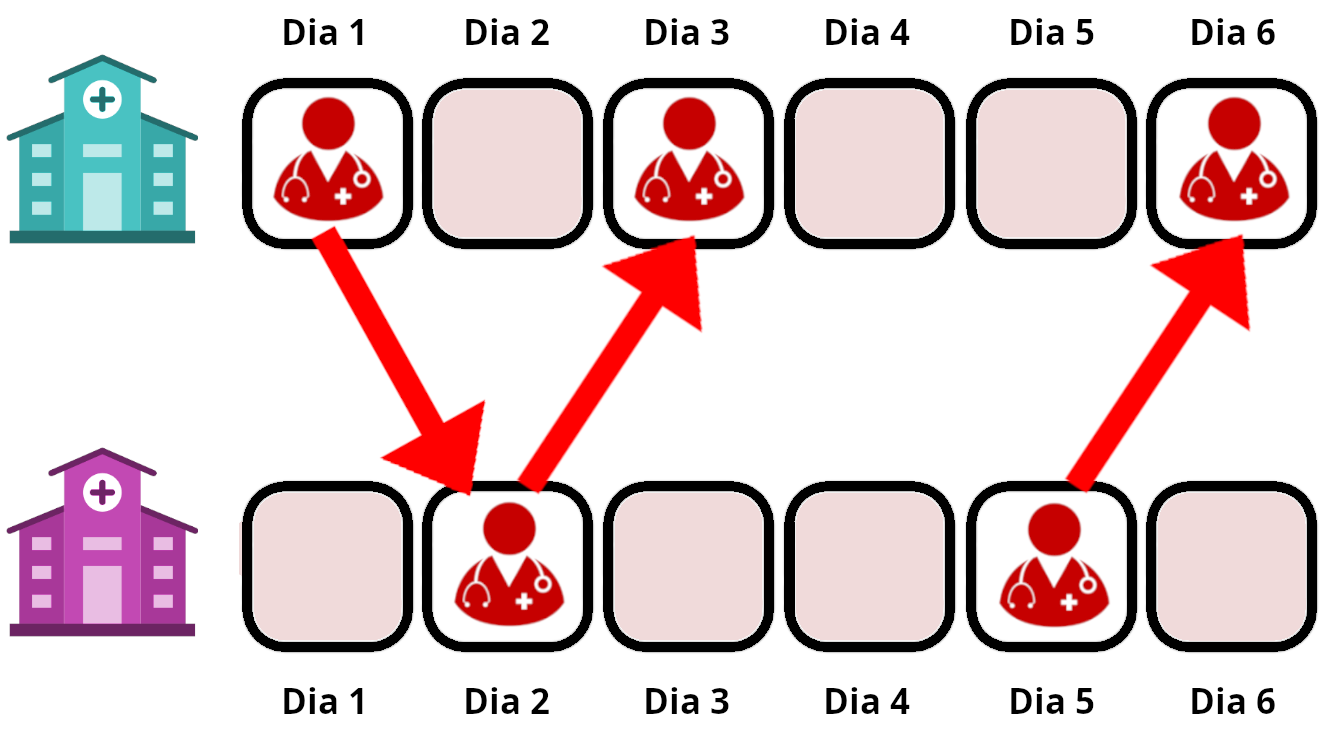
\includegraphics[width=\linewidth]{img/troca-examplo.png}
                \caption{Troca $=$ mudar de unidade entre dias.}
                \label{fig:ex-troca}
            \end{figure}
        \end{column}
    \end{columns}
    % TODO: objetivos conflitantes -> motiva fronteira de Pareto (Seção 3).
\end{frame}

%%% Frame 2.6 — Variável de estado gamma (contribuição de modelagem)
\begin{frame}{Detectando trocas}
    \begin{columns}[T]
        \begin{column}{0.55\textwidth}
            \begin{block}{Problema}
                Lacunas (dias sem trabalho) quebram a comparação ingênua de $w$ entre dias consecutivos.
            \end{block}
        \end{column}
        \begin{column}{0.5\textwidth}
            \resizebox{\linewidth}{!}{\begin{minipage}{1.15\linewidth}
                {\small
                \begin{alignat}{2}
                    \gamma_{iud} &\geq w_{iud} \label{eq:g-def} \\
                    \sum_{u \in U_i} \gamma_{iud} &= 1 \label{eq:g-sum} \\
                    z_{id} &\geq \gamma_{iud} + \!\!\sum_{u' \neq u}\! \gamma_{i,u',d-1} - 1 \label{eq:g-swap}
                \end{alignat}
                }
                {\centering\tiny $\gamma_{iud}$ adaptado do GLSP~\cite{Fleischmann_Meyr_1997}.\par}
            \end{minipage}}
        \end{column}
    \end{columns}
    \begin{center}
        \begin{figure}
            \centering
            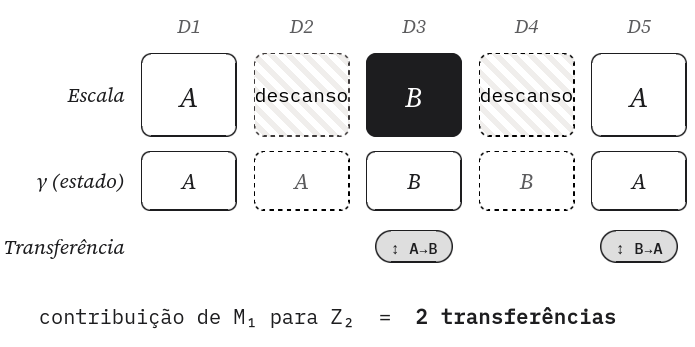
\includegraphics[width=0.7\linewidth]{img/04_nsga-05_gama.png}
            \caption{Estado $\gamma$ persiste nas lacunas.}
            \label{fig:gamma}
        \end{figure}
    \end{center}
\end{frame}
